% CSCI3753 - Operating Systems
% Spring 2012
% Programming Assignment 3
% By Andy Sayler (3/6/12)

\documentclass[12pt]{article}

\usepackage[text={6.5in, 9in}, centering]{geometry}
\usepackage{graphicx}
\usepackage{url}

\title{Programming Assignment 3:\\Investigating the Linux Scheduler}
\author{
  CSCI 3753 - Operating Systems\\
  University of Colorado at Boulder\\
  Spring 2012\\
  By Andy Sayler and Junho Ahn and Richard Han
}
\date{\emph{Due Date:  Friday, March 23, 2012 11:55pm}}

\begin{document}

\maketitle

\section{Assignment Introduction}

The goal of this assignment is to spend some time investigating the
behavior of the Linux scheduler. You will create a set of benchmarks
and run them under a variety of Linux scheduling polices. You will
then use the data from these benchmarks to draw some conclusions about
the differences between the various Linux scheduler polices. You will
submit a report explaining your conclusions and showing your
supporting data.

You may complete this assignment on the course VM or your own native
Linux 2.6.32+ installation. You will not be able to complete this lab
directly on the CU CSEL or elra machines as you will require super
user access in order to utilize certain scheduler policies.
You will probably get the most reliable data off of a personal, native
Linux install with few other programs running simultaneously. Whatever
environment you chose to use must be used consistently throughout this
assignment. Switching environments part way through The assignment
will make it difficult, if not impossible, to accurately compare and
contrast your data. Be sure to document your environment in your
report.

\section{The Linux Scheduler}

The current implementation of the Linux
Scheduler has existed since kernel version 2.6.23 when the Completely
Fair Scheduler (CFS) was added to the mainline Linux kernel
\cite{Molnar-CFS,Jones-InsideCFS,Kumar-MultiCFS}. Prior to kernel
version 2.6.23, Linux used the O(1) scheduler \cite{Le-StudyLKS}.
This assignment will focus on the current scheduler implementation.

The addition of the CFS scheduler to the Linux kernel brought with it
a more modular scheduler implementation. The scheduler is implemented as
a core unit (\texttt{kernel/sched.c}) that implements the core
scheduler behavior and a serious of scheduler class modules that
implement specific scheduling policies. Currently, the kernel contains
two of these scheduler classes: The CFS class
(\texttt{kernel/sched\_fair.c}) and the Real Time (RT) class
(\texttt{kernel/sched\_rt.c}). These classes are
organized hierarchically,
with the RT class taking precedence over the CFS class. The scheduler
core attempts to schedule all runnable jobs from each class before
moving on to the next class in the hierarchy.

\begin{figure}[htbp]
  \begin{center}
    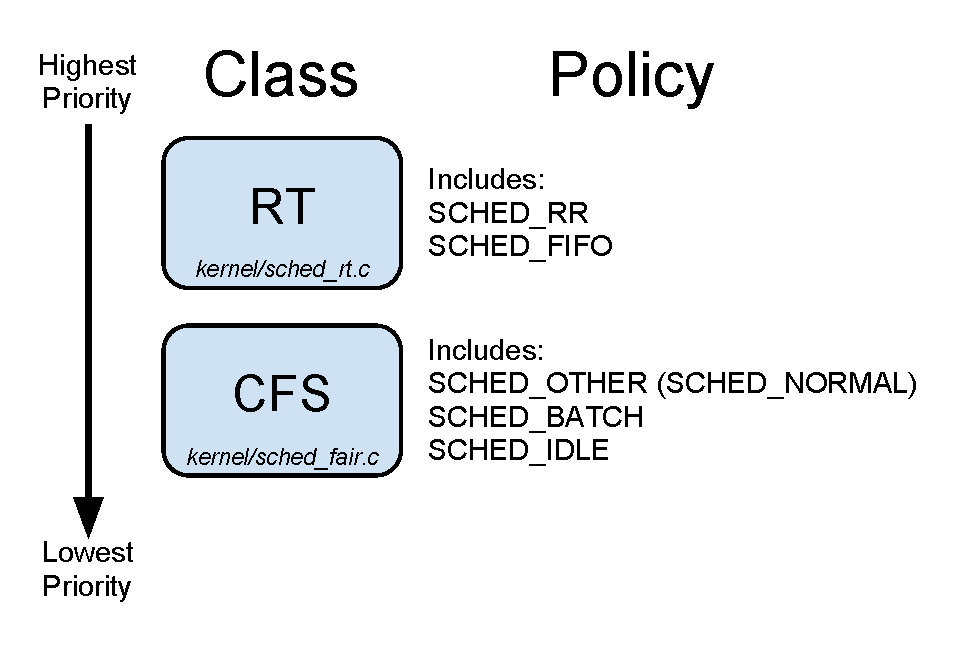
\includegraphics[scale=.9]{LinuxSchedulingClass.pdf}
    \caption{Linux Scheduling Classes and Policies}
    \label{fig:LSClasses}
  \end{center}
\end{figure}

Each scheduler class implements one or more scheduler policies. Each
policy controls the scheduling behavior of all system processes
assigned to it. The RT class currently provides implementations of the
POSIX SCHED\_RR and SCHED\_FIFO policies. The CFS class currently
provides implementations of the SCHED\_OTHER (aka SCHED\_NORMAL),
SCHED\_BATCH, and SCHED\_IDLE policies. The default policy is
SCHED\_OTHER. Polices within a given class may or may not posses a
hierarchical relationship. It is up to each class to determine how it
handles any polices it implements. See Figure \ref{fig:LSClasses}. 

\begin{figure}[htbp]
  \begin{center}
    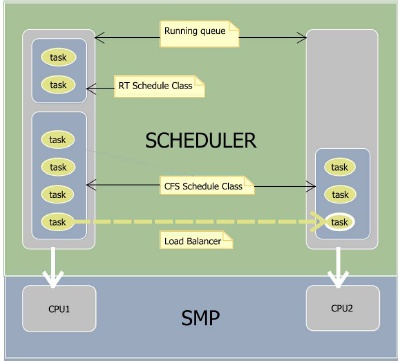
\includegraphics[scale=.75]{LinuxSchedulerOverview.jpg}
    \caption{Linux Scheduler Overview \cite{Le-StudyLKS}}
    \label{fig:LSOverview}
  \end{center}
\end{figure}

In Linux, each processor has its own run queue structure. Originally this
structure was a single queue that maintained a list of processes for
each processor to run (hence the name ``run queue'').
Today, this structure actually contains a collection of
sub-structures (or pointers to sub-structures),
where each sub-structure corresponds to the necessary
data structure(s) for each scheduling class. Since Linux currently
has two scheduling classes, CFS and RT, each run queue structure
contains a pointer to a CFS run queue structure and a RT run queue
structure. These
run queue structures are managed by their respective scheduling
classes. Also, note that although we still use the phrase ``run queue''
many of these structures are no longer actually queues. For instance, the CFS
class uses a Red-Black Tree as its so called ``run queue''. We will
use the term ``run queue'' in this wider since to refer to any data
structure that a class uses to organize or derive a scheduling order for a
set of processes.

In a Linux SMP multiprocessor installation there is one set of run queue
structures per processor (or core). This means there must also be
a load balancing system
to move tasks from one run queue to another. Like the rest of the
scheduling system, load balancing is handled separately by each
scheduling class. Figure \ref{fig:LSOverview} provides an illustration
of the organization of the scheduling system.

The scheduler core is coordinated by a series of regular,
frequent ticks. Each tick, the scheduler attempts to find a runnable
process for each available core on each available processor. As
mentioned previously, the scheduler accepts processes from each class
in order of the class hierarchy. The scheduler core calls a function
hook in each scheduler class called \texttt{pick\_next\_task}, passing
this function a copy of the run queue structure corresponding to the
processor currently being scheduled. Each scheduler class then accesses its
corresponding sub-structure within the run queue structure and performs
the necessary computation to arrive at the appropriate next task. It then
passes a pointer to the \texttt{task\_struct} for this task back to the
scheduler core for
running. If a class has no runnable processes, it returns a NULL
pointer and the scheduler moves on to the next class in the hierarchy.

Scheduler polices are used within each class to indicate a desired
scheduling behavior. By convention, if multiple polices can share a run
queue data structure, they are implemented in the same class. The
default policy, \texttt{SCHED\_OTHER} (also called
\texttt{SCHED\_NORM}) corresponds to the standard CFS time-sharing
scheduling parameters. The two RT policies, \texttt{SCHED\_FIFO} and
\texttt{SCHED\_RR} implement real-time first-in-first-out and real-time
round-robin scheduling policies, respectively. It should be noted that
the ``real-time'' policies in Linux are soft real-time polices, as
Linux is not a hard real-time operating system. This means that Linux
will make a best effort to adhere to real-time scheduling rules for
these policies, but can not guarantee it. Each task assigned to a RT
policy must be given a scheduling priority. These priorities dictate the
ordering of tasks in the real-time run queue. The CFS class does not
use user supplied scheduling priorities.

\section{Process Types}

In general, we speak of processes as being either compute bound, or
I/O bound. A compute, or CPU, bound process is a process that primarily
requires use of the CPU in order to complete. The speed and availability
of the CPU is the limiting
factor determining the run time of such a process.

An I/O bound process, on the other hand, is a process that
primary relies on completing I/O requests (hard disk, user input, etc)
in order to complete. The run time of an I/O bound process is primary
determined by the amount of time it must spend waiting for I/O
resources to become available.

In reality, most programs lie somewhere in between these two
extremes. But it is helpful to consider these extremes when analyzing
the speed and behavior of a process.

\section{Your Task}

This project requires you to complete the following three items:

\begin{itemize}
\item Design a series of benchmarks to evaluate the behavior of
  several scheduling polices in the linux scheduler.
\item Run your benchmarks and analyze the resulting data to draw
  conclusions about the behavior of the tested policies. 
\item Write a report explaining your conclusions and supporting data.
\end{itemize}

Each item is discussed in detail below.

\subsection{Create Benchmarks}

You will need to benchmark and analyze the behavior of the following
three Linux Scheduling policies:

\begin{itemize}
\item \texttt{SCHED\_OTHER} (aka \texttt{SCHED\_NORM})
\item \texttt{SCHED\_FIFO}
\item \texttt{SCHED\_RR}
\end{itemize}

You will need to compare the behavior of these polices across the
following three representative process types:

\begin{itemize}
\item Compute (CPU) Bound
\item I/O Bound
\item Mixed
\end{itemize}

Additionally, you will need to investigate how the behavior of each
process type under each scheduling policy scales across the following
three levels of system utilization:

\begin{itemize}
\item Low (5 to 10 simultaneous process instances)
\item Medium (10s of simultaneous process instances)
\item High (100s of simultaneous process instances)
\end{itemize}

\subsection{Run and Analyze}

The three testing vectors mentioned above give rise to 27 possible
test cases (every possible combination of each of the three elements
from each of the three vectors). You will need to gather data for all
27 of these cases. You should probably also repeat each
test case a few times and average the results over this set
of runs. This will help insure that you are getting good data and
will minimize the effect of spurious events.

Once you have gathered all of your data, you will need to analyze it
to answer the following questions:

\begin{itemize}
\item Which scheduling policy is best suited for each process type in
  terms of run-time and overhead efficiency?
  Why? If there is not a clear winner, why not?
\item How does each scheduling policy scale? Why?
\item What are some pros and cons of each scheduling policy?
\item Provide an example of an instance for which each scheduling
  policy is well suited.
\item Provide an example of an instance for which each scheduling
  policy is not well suited.
\end{itemize}

\subsection{Report}

Write a report that explains how you gathered your data, what your
data show, and why you believe you obtained the results that you did. Work
the answers to the above questions into your report. The questions
need not be answered directly, but the reader should be able to answer
all of the questions posed above after reading your report.

Your report must include the following section:

\begin{itemize}
\item Abstract - A single paragraph overview of your work and conclusions
\item Introduction - An overview of your work
\item Method (or Experimental Design) - An explanation of how your
benchmarks work and what they test for. You should also describe your
test system and setup.
\item Results - Summary of your results (possibly with graphs)
\item Analysis - Explanation of your results and what they indicate
\item Conclusion - What you learned from your results
\item References - Any external resources you consulted
\item Appendix A - Raw Data
\item Appendix B - All Code
\end{itemize}

The report should be no longer than necessary to effectively convey your
meaning. Excluding the Appendices, 10 pages would seem a reasonable
upper limit, but adjust as necessary. The report should be written in
active, first person English and should adhere to the standards of good
writing \cite{StrunkWhite,K&R}. References may be in any format you chose,
as long as they convey the point.

Assume that your audience is educated in the subject
(i.e. the course TAs or professor). Thus, you need not dwell on
background information. Concentrate on explaining the unique properties of
your work (your benchmark implementation, etc), your results, and your
conclusions.

This document is a reasonable example of the writing
style and quality level for which we are looking. If you require
additional examples of ``good'' reports, please contact the TAs.

\section{Some Implementation Ideas}

There are a variety of ways you could meet the requirements of the
assignment listed in the previous section. Here we provide suggestions
for a few possible ways.

\subsection{Create Test Programs}

To create test programs for the three required process types,
write a simple C program implementing
each. For example, the compute bound program might involve
calculating pi to the nth digit or generating a pseudo-random number.
Algorithms for these and other CPU
heavy tasks can be found online and in reference texts.

To create an
I/O bound program, consider writing a program that writes B bytes to a
file, and then reads the B bytes back from the file, repeating N
times. You may need to pick B and N such that you can overcome the
caching effects of the system in order to get the best data. The Linux
\texttt{/dev/null} and \texttt{/dev/urandom} files may come in handy
if you wish to throw data away or read random data. Be wary of
accessing a common file in your program, as you will need to be
able to run multiple copies of your program simultaneously to get
accurate benchmark results. If your program must read in or write out
to a file, it would be best to create a separate input/output files for
each instance of your program.

For a mixed program, combine the previous ideas. For example, carry out a
computationally heavy step in an algorithm, write the intermediate
result to a file, and then repeat N times.

Once you have your three programs implementing the three process types,
modify the program so that it spawns N instances of itself. You will
need to utlize the \texttt{fork} system call in order to spawn
additional programs. You should probably structure the program to
maintain a single parent process that spawns and monitors all
children. Your children processes will then carry out the necessary
work for the given test program as discussed above.
You will need to make sure that your parent process waits on
each child to insure they are properly reaped, avoiding zombie
processes. This becomes especially important when you start gathering data,
as you will not be able to properly collect performance metrics from
zombie processes. 

In order to set the scheduling policy for a process, you will need to
use the \texttt{sched\_setscheduler} system call. If called at the start
of each of your test programs, the appropriate scheduling policy
will be inherited by any forked children within the program. You must pass
\texttt{sched\_setscheduler} a priority level when you call it.
The \texttt{SCHED\_OTHER} priority should always be
0. \texttt{SCHED\_RR} and \texttt{SCHED\_FIFO} should have priorities
greater than 0, but should be the same for all tests so that process
priority is not a factor in your benchmark results. You may use the
\texttt{sched\_get\_priority\_max} function to find the max priority a
given schedule policy supports. In addition, the RT scheduling
polices can only be run by a privileged user. Thus, you will need to
use the \texttt{sudo} command to run any benchmark that uses a RT
scheduling policy.

Using the above steps, you can write a generalized version of each
of the three necessary test programs that takes as arguments the
scheduler class and
the number of copies to spawn (and, if desired, some measure of the
amount of time, number of iterations, etc that it should run each copy).
You could then write a script that calls each program with the
appropriate parameters to generate test runs
across the 27 different combinations of test values. Remember, the
computer works for you, not the other way around.

Note that you
should wait for each specific test case to complete before
starting the next. You will adversely intertwine your results if you
run multiple tests simultaneously. Also note that you will
need a minimum value of 5 to 10 simultaneous copies (children) of each test
program running simultaneously to get interesting results. If only a
single instance (child) of each test program is running at a time, all of the
scheduling policies will behave in the same manner since there is
nothing to schedule.

\subsection{Measure Program Performance}

The previous section focused on building benchmark programs, but does
not include any info on actually gathering data on the performance of
these programs. Linux provides a number of ways to collect metrics on
a program's performance. We discuss a few here.

The simplest means of collecting performance metrics is to use the Linux
\texttt{time} command. The GNU version of this command returns a
wealth of data about a program, including the system time, user time,
real time, and number of context switches. All of this data can be
used to gain insights into the behavior of the various scheduling
classes. With proper scripting, you can even automatically collect and
average this data over several test runs of each test case.

The upside to using \texttt{time} is that you may apply it directly to each of
the test programs you have built, without needing to modify any of the
test code discussed above (except maybe the top level script).
The downside to using the \texttt{time} command is that you will only be able to gather
the total aggregate data for each test case. You will not be able to gain any
insight into the fine grain distribution of this data across each
specific child instance. Assuming your test program properly waits
on any children that it spawns, the results returned by \texttt{time}
will be the sum of the results from the parent process and any
descendants. You can use this to compute the average resource usage of
each test program child instance by dividing the results by the number
of instanced spawned in a given test case.
This averaged data may be fine for your
purposes, or it may leave you needing finer grain data.

If you want to gather the same data that \texttt{time} can give you,
but for each individual child process instance, you can use the
\texttt{getrusage} or \texttt{wait4} system calls. Unlike
\texttt{time}, these function will need to be built
directly into your test programs. They will, however allow you to
gather data on each individual child process as it finished and is
reaped. If using \texttt{getrusage}, you may have to setup
the necessary signal handlers to insure it gets
called each time a child process exits. If using \texttt{wait4}, you
can gather statistics on each child process as it is reaped.

It may be wise to start by
using the \texttt{time} command and to only add \texttt{getrusage} or
\texttt{wait4} if you feel you need it. Alternatively, if you are
uncomfortable with a scripting language and do not wish to record your
results by hand, you could use \texttt{getrusage} or \texttt{wait4} to
collect and process all necessary data inside a top level c program.

\section{What You Must Provide}

When you submit your assignment, you must provide the following as a
single archive file:
\begin{itemize}
\item A copy of your report in pdf format
\item A copy of all your test code
\item A makefile that builds any necessary test code
\item A README explaining how to build and run your code
\end{itemize}

\section{What's Included}

We provide some code to help get you started. Feel free to use it as a
jumping off point (appropriately cited).

\begin{enumerate}

\item {\bf pi.c} The source code for a statistically-based pi
  calculator. Accepts as the first argument the number of iterations to
  compute over. Example of a CPU bound process.

\item {\bf pi-sched.c} Same as pi.c, but with the addition of the
  ability to select one of the following three Linux scheduling
  policies: SCHED\_OTHER, SCHED\_RR, or SCHED\_FIFO. Accepts a scheduling
  policy as the second argument.
\emph{Note 1: Only privileged users can
  utilize the RT SCHED\_RR and SCHED\_FIFO policies.}
\emph{Note 2:
    Neither pi or pi-sched spawns multiple instances. This is
    functionality you will need to add if you wish to use these
    programs as part of your test suite}

\item {\bf testscript} A simple bash script that runs and measures the
  performance of a single instance of the pi-sched program across all
  three scheduling policies.

\item {\bf rw.c} The source code for a simple program that copies N
  bytes in blocks of K bytes
  from an input file to an output file. The program will read the input
  file multiple times in order to generate the required number of N
  bytes when N is larger than the size of the input file. Uses the
  low-level \texttt{read} and \texttt{write} system calls
  in the \texttt{O\_SYNC}
  mode to minimize the effects of filesystem buffering and maximize
  I/O delays. Example of an I/O bound process.

\item {\bf Makefile} A GNU Make makefile to build all the code listed
  here.

\item {\bf README} As the title so eloquently instructs: read it.

\end{enumerate}

\section{Extra Credit}

There are a few options for receiving extra credit on this
assignment. Completion of each of the following will gain you the
specified number of points. In no case will the maximum score on
this assignment exceed 110/100.

\begin{itemize}
\item {\bf BFS}: The BFS is an alternative to the
  CFS. It is actively maintained as a set of patches that
  can be found at
  \url{http://ck.kolivas.org/patches/bfs/}
  \cite{Kolivas-BFS,Kolivas-BFSFAQ}. Patch
  and recompile a copy of the Linux kernel that uses the BFS instead
  of the CFS. Run all of the required test combinations in the BFS
  kernel, as well as in the CFS kernel (bringing your total test cases
  to 54). Compare the performance of the BFS and CFS policy
  implementations in your
  report. {\bf 10 Points} \emph{Bonus: Fame. If you do this well, there may
  be a demand for your report online or in publication. There has been
  a lot of speculation on the relative performance of CFS vs BFS but not
  much comprehensive data to back it up.}
\item {\bf Visualization}: Build or deploy a visualization system that
  will create visual representations of how various scheduling polices
  schedule the different tasks. Your output might look like the
  Gantt charts we have looked at in recitation and class. You will
  probably have to use some form of process trace library to gather the
  necessary temporal data. {\bf 10 Points}
\item {\bf Multi-Core}: Investigate how the various scheduling polices
  scale with the number of cores. You will essentially need to add core
  count as an additional test parameter (multiplying the total number
  required test
  results in the process). Compare the performance of the various
  scheduling policies on single, double, and quad or more core machines and
  comment on the results in your report. A virtualized environment
  would seem the best suited for this extension. {\bf 10 Points}
\end{itemize}

\section{Grading}

40\% of you grade will be based on the submission you provide.
To received full credit your submission must:
\begin{itemize}
\item Meet all requirements elicited in this document
\item Code must build with ``-Wall'' and ``-Wextra'' enabled,
  producing no errors or warnings.
\item Report must be well written and reasoned.
\end{itemize}

The other 60\% of your grade will be determined via your grading
interview where you will be expected to explain your results and answer
questions regarding them and any concepts related to this assignment.
This includes adhering to good coding style and writing practices.

\section{Obtaining Code}
The starting code for this assignment is available on the Moodle and
on github. If you would like practice using a version control system,
consider forking the code from github. Using the github code is not
a requirement, but it will help to insure that you stay up to date
with any updates or changes to the supplied codebase. It is also
good practice for the kind of development one might expect to do in
a professional environment. And since your github code can be easily
shared, it can be a good way to show off your coding skills to
potential employers and other programmers.

Github code may be forked from the project page here:\\
\url{https://github.com/asayler/CU-CS3753-2012-PA3}.

\section{Resources}
Refer to your textbook and class notes on the Moodle for an overview
of OS scheduling policies and implementations.

The Internet\cite{tubes} is also a good resource for finding
information related to solving this assignment.

You may wish to consult the man pages for the following items, as they
will be useful and/or required to complete this assignment. Note that
the first argument to the ``man'' command is the chapter, insuring
that you access the appropriate version of each man page. See
\texttt{man man} for more information.

\begin{itemize}
\item \texttt{man 1 time}
\item \texttt{man 2 sched\_setscheduler}
\item \texttt{man 2 sched\_get\_priority\_max}
\item \texttt{man 2 getrusage}
\item \texttt{man 2 ptrace}
\item \texttt{man 2 fork}
\item \texttt{man 2 wait}
\item \texttt{man 2 wait4}
\item \texttt{man 2 open}
\item \texttt{man 2 close}
\item \texttt{man 2 read}
\item \texttt{man 2 write}
\item \texttt{man 4 random}
\item \texttt{man 4 null}
\item \texttt{man 5 proc}
\item \texttt{man 7 sched.h}
\end{itemize}

\begin{thebibliography}{9}

\bibitem{Jones-InsideCFS} Jones, M. Tim.
  \newblock \emph{Inside the Linux 2.6 Completely Fair Scheduler}.
  \newblock IBM developerWorks: 2009.
  \newblock Accessed 06/01/12.
  \newblock \url{http://www.ibm.com/developerworks/linux/library/l-completely-fair-scheduler/}.

\bibitem{K&R} Kernighan, Brian and Dennis, Ritchie.
  \newblock \emph{The C Programming Language}.
  \newblock Second Edition: 2009.
  \newblock Prentice Hall: New Jersey.

\bibitem{Kolivas-BFS} Kolivas, Con.
  \newblock \emph{BFS - The Brain Fuck Scheduler}.
  \newblock 2009.
  \newblock Accessed 06/01/12.
  \newblock \url{http://ck.kolivas.org/patches/bfs/sched-BFS.txt}.

\bibitem{Kolivas-BFSFAQ} Kolivas, Con.
  \newblock \emph{FAQS about BFS}.
  \newblock v0.330: 2009.
  \newblock Accessed 06/01/12.
  \newblock \url{http://ck.kolivas.org/patches/bfs/bfs-faq.txt}.

\bibitem{Kumar-MultiCFS} Kumar, Avinesh.
  \newblock \emph{Multiprocessing with the Completely Fair Scheduler}.
  \newblock IBM developerWorks: 2008.
  \newblock Accessed 06/01/12.
  \newblock \url{http://www.ibm.com/developerworks/linux/library/l-cfs/}.

\bibitem{Le-StudyLKS} Le, Thang Minh.
  \newblock \emph{A Study on Linux Kernel Scheduler: version 2.6.32}.
  \newblock 2009.
  \newblock Accessed 06/01/12.
  \newblock \url{http://www.scribd.com/thangmle/d/24111564-Project-Linux-Scheduler-2-6-32}.

\bibitem{Molnar-CFS} Molnar, Ingo.
  \newblock \emph{This is the CFS scheduler}.
  \newblock 2007.
  \newblock Accessed 06/01/12.
  \newblock \url{http://people.redhat.com/mingo/cfs-scheduler/sched-design-CFS.txt}.

\bibitem{tubes} Stevens, Ted.
  \newblock \emph{Speech on Net Neutrality Bill}.
  \newblock 2006.
  \newblock \url{http://youtu.be/f99PcP0aFNE}.

\bibitem{StrunkWhite} Strunk, William, Jr. and White, E.B.
  \newblock \emph{The Elements of Style}.
  \newblock Fourth Edition: 2000.
  \newblock Pearson: New York.
  
\end{thebibliography}

\end{document}  
